\documentclass[a4paper,10pt]{article}
\usepackage[utf8]{inputenc}
\usepackage{natbib}
\usepackage{graphicx}% Include figure files
\usepackage{amsmath}


\newcommand{\inblue}[1]{{\color{blue}#1}}
\newcommand{\inred}[1]{{\color{red}#1}}

%opening
\title{Coherence vortices in the Cross Spectral Density. Something to consider in diffraction and imaging?}
\author{Manuel Sanchez del Rio$^1$, David Paganin$^2$}

\begin{document}

\maketitle

\begin{abstract}

\end{abstract}

\section{What is the Cross Spectral Density (CSD)?}

It is the function that measures the correlation of the electric disturbance between two points.

\begin{equation}
W(x_1,y_1,x_2,y_2,z,\omega) = 
\langle E^{*}(x_1,y_1,z,\omega) E(x_2,y_2,z,\omega)\rangle.
\end{equation}

The CSD quantifies the two-point correlation properties of a partially coherent statistically stationary source \cite{Wolf1982,mandel_wolf}. 
It is the input input needed to properly model any subsequent x-ray data obtained by streaming such CSD through subsequent optical elements, samples, and detector.

Recall that the cross-spectral density $W$, spectral density $S$ and mutual coherence function (normalized CSD) $\mu$ are related by $W(r_1,r_2,\omega)=\sqrt{S(r_1,\omega)}\sqrt{S(r_2,\omega)}\mu(r_1,r_2,\omega)$. 

In this work, we consider the role played by the phase of CSD. It governs the position of Young-type interference fringes formed when the disturbance from two different spatial points is combined. It influences the detected intensity in both imaging and non-imaging experiments.

\begin{equation}\label{phase_of_W}
\Phi(x_1,y_1,x_2,y_2,z,\omega)=\arg[W(x_1,y_1,x_2,y_2,z,\omega)]
\end{equation}




\section{What is a vortex?}


\begin{figure}\label{loss_of_fringe_visibility}
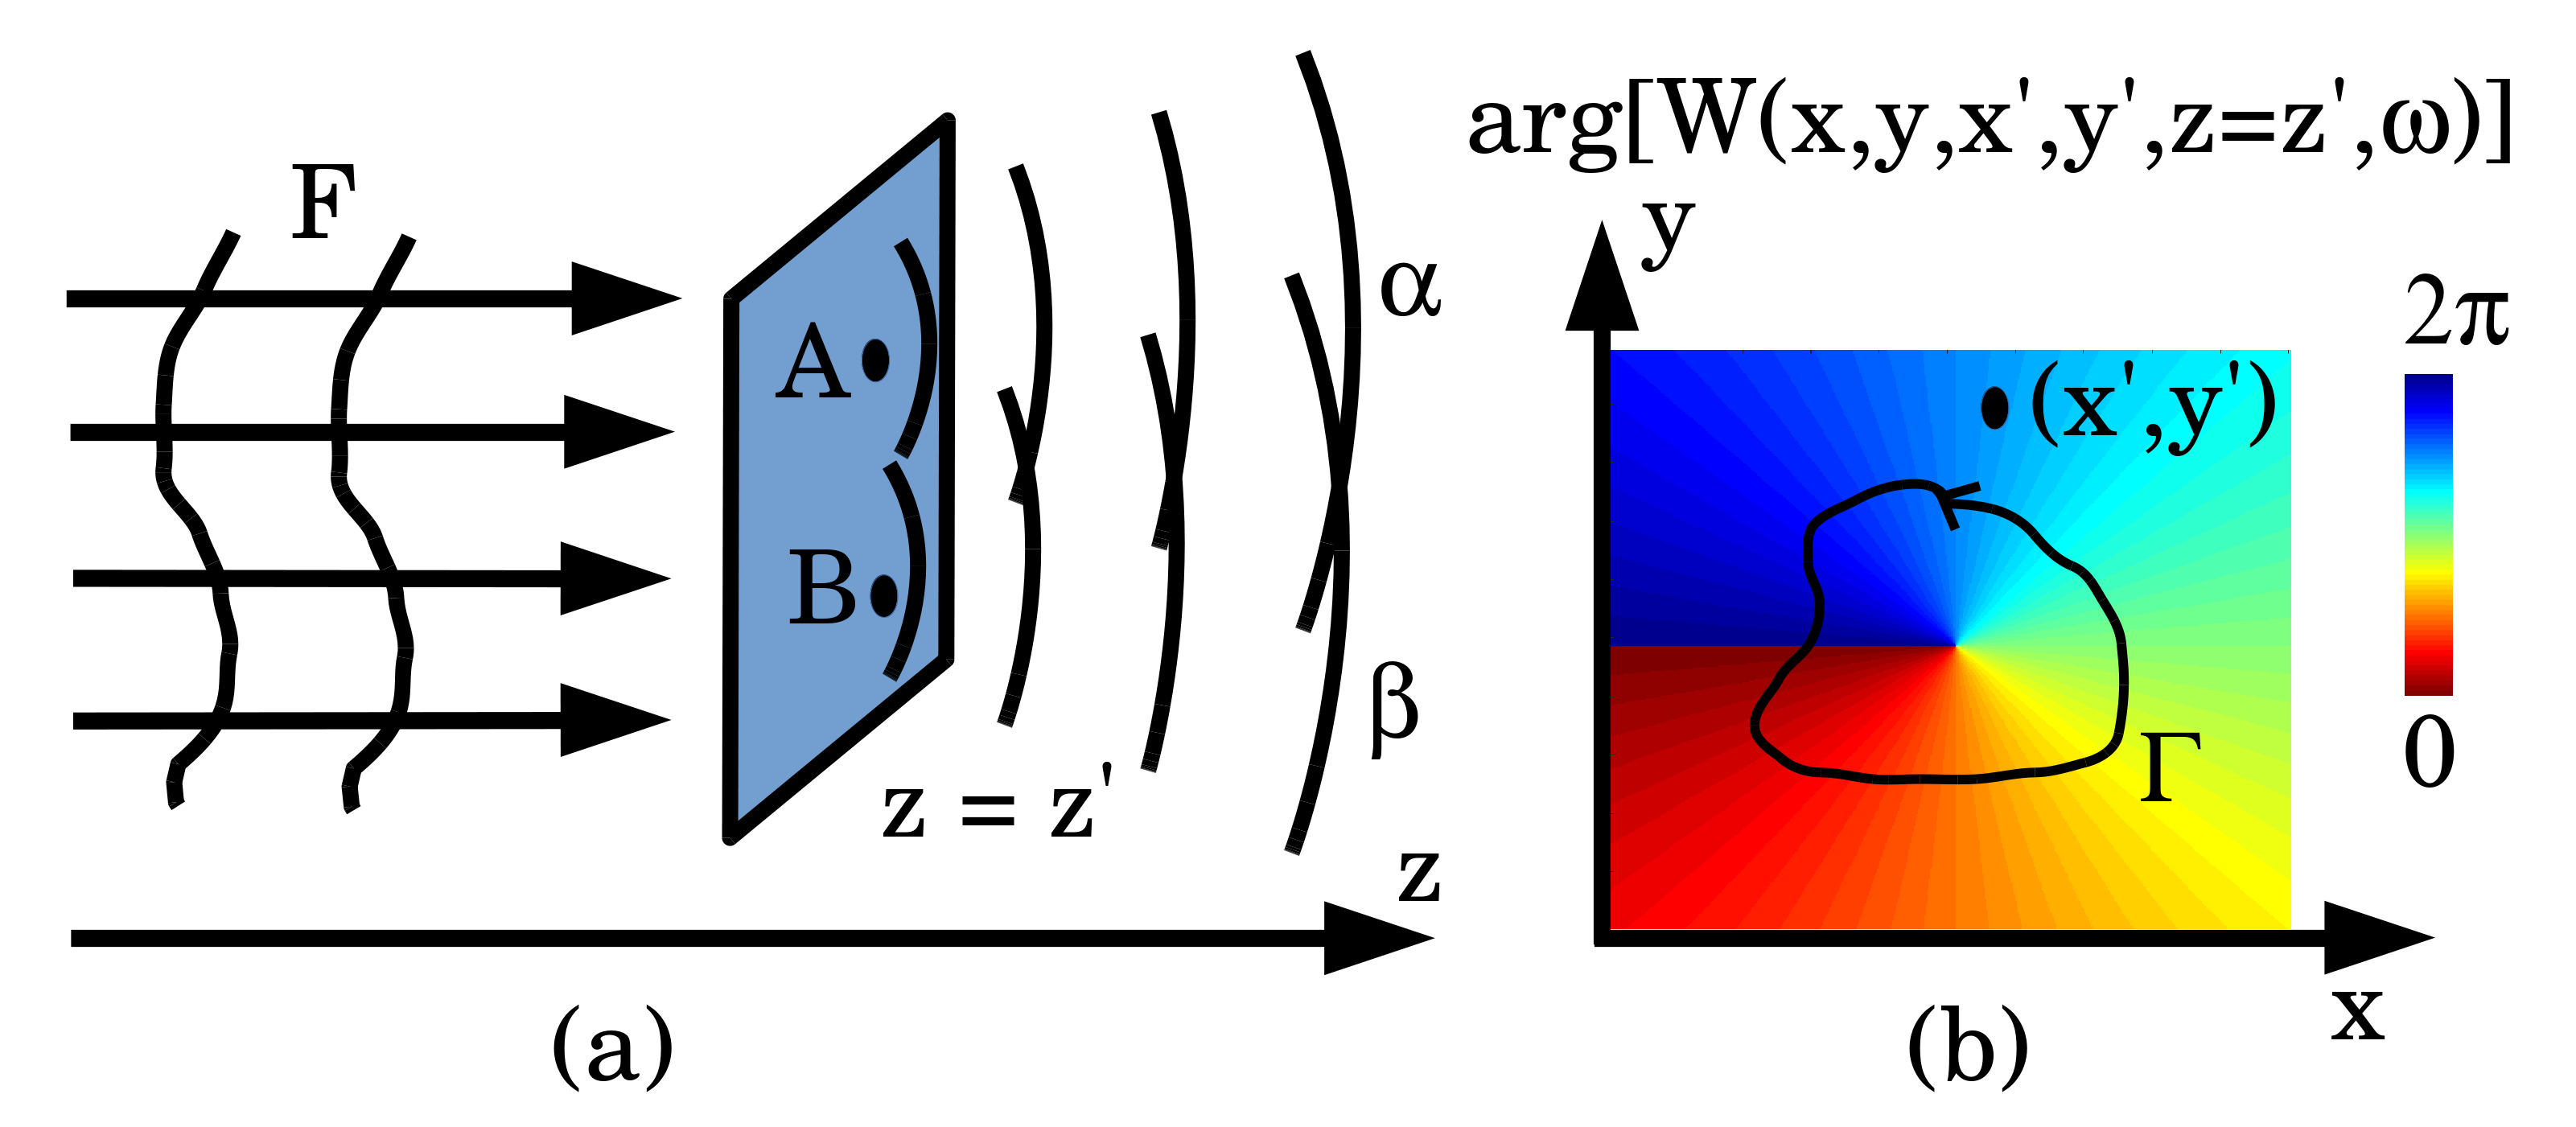
\includegraphics[width=0.45\textwidth]{Figures/coherence_vortex.png}
\end{figure}
 
 
$W$ is single-valued, but $\Phi$ will in general be multi-valued. Indeed, since the phase of a complex number is only defined modulo $2\pi$ radians, it may wind by an integer multiple of $2\pi$ in the following manner (see Fig.~\ref{loss_of_fringe_visibility}b) \cite{GburVisser2003}: 
\begin{equation}
\label{phase_of_W_winding}
\oint_{\Gamma} d\Phi(x_1,y_1,x_2,y_2,z,\omega)=2\pi m.
\end{equation}
Here, $\Gamma$ is any smooth closed curve (see Fig.), $m$ is an integer and $d\Phi$ is the increment in $\Phi$ corresponding to an infinitesimal line segment of $\Gamma$.
A non-zero $m$ indicates the presence of non-trivial topology in the phase of $W$, thus a coherence vortex \cite{GburVisser2003} is present.  

\section{What do a vortex imply?}

The existence of any {\em one} circuit $\Gamma$ for which $m$ is non-zero, implies the presence of a (nodal) manifold of points in $(x_1,y_1,x_2,y_2,z,\omega)$-space, at each of which $W$ vanishes. These nodal points in $W$ exhibit ``complete destructive interference of coherence''. If, for example, a point scatterer were to be placed at $A$, with another point scatterer at $B$, and the radiation scattered from both points allowed to overlap, no interference fringes would be observed if the resulting diffracted fields were to be filtered to angular frequency $\omega'$.

\begin{figure}\label{Young_fringe_anholonomy}
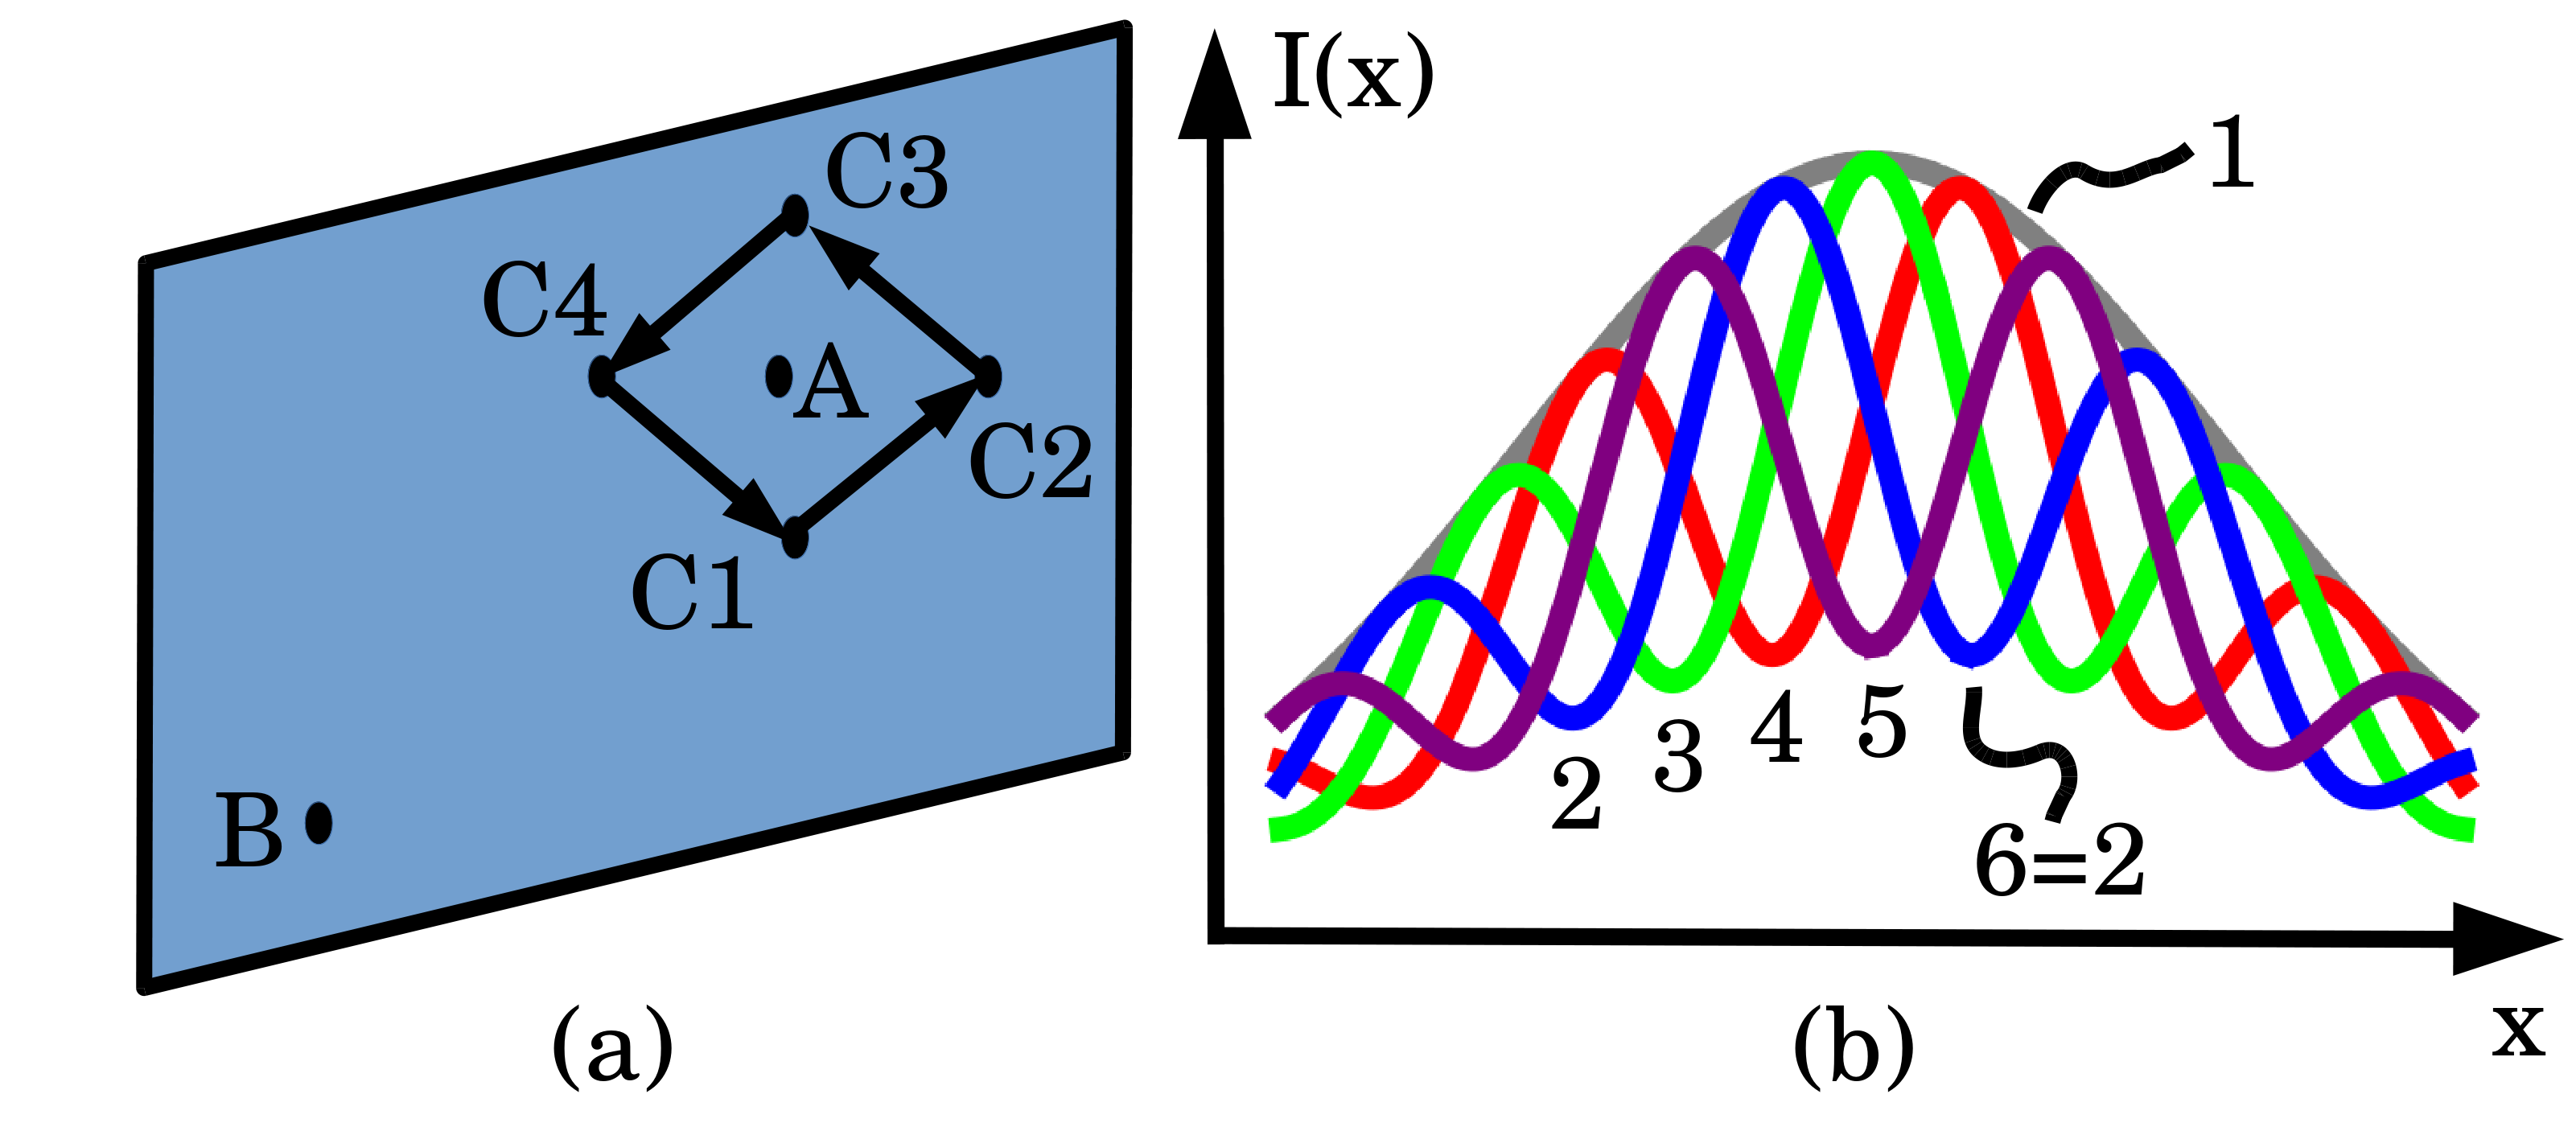
\includegraphics[width=0.7\textwidth]{Figures/Anholonomy.png}
\end{figure}
 
The vortical nature of the coherence vortex is manifested if one performs a sequence of Young-type interference experiments, where the pinhole at $B$ is kept fixed, while the pinhole at $C1$ is moved through the cycle of locations $C1$ (curve 2), $C2$ (curve 3), $C3$ (curve 4), $C4$ (curve 5) and finally back to $C1$ (curve 6 = curve 2). If one traces the evolution of the intensity maxima associated with the sequence of Young-type interferograms in curves 2 to 6, the physical meaning of $m$ becomes clear: during the cycle, if $m=1$ then the maxima of the interferogram will ``ratchet'' to the right by one fringe during the cycle. If $m=-1$ they would instead ratchet to the left by one fringe during the cycle.  For general $m$, the fringes would ratchet to the right (left) by $|m|$ fringes, if $m$ is positive (negative).
 
 
\section{Do we expect coherence vortices in our synchrotron beams}

Yes. As far as the beam is partial coherent, there are vortices. The number of vortices depend on the coherent fraction. More coherence imply less vortices, but their effect is more visible in a potential experiment. We make a theoretical-numeric study here of the vortices in a synchrotron beam to be produced by EBS.


\section{How to calculate the phase of the CSD to look for vortices?}

We use COMSYL to calculate the CSD as a function of the coherent modes using :


\begin{equation}
W(\vec{r_1}, \vec{r_2}, \omega)
=
\sum_m
\lambda_m(\omega)
\phi_m^*(\vec{r_1},\omega)
\phi_m(\vec{r_2}, \omega).
\end{equation}

We analyzed the case if a U18 undulator at 17 keV. We need about 1000 modes to represent 97.9\% of the intensity. Later on, the beamline optics will reduce the number of modes  with a subsequent reduction of intensity. In a beamline some optical elements (ideal reflectors, ideal focusing elements) do not alter the occupation spectrum of the modes. They are non-absorbing or conservative elements in the sense of Smith-Helmholtz invariant. However, if an optical element remove photons from the beam, or ``cuts'' intensity, then its effect is different on the different modes. The new transformed ``modes'' can be used to build the CSD, but they cannot be considered coherent modes as they are not longer an orthonormal basis for expanding the CSD. A new coherent mode decomposition could be calculated on the transmitted CSD in order to obtain the new coherent modes. In the case of slits or pinholes centerd on the optical axis, the lower coherent modes localised near the center of the beam axis will propagate, whereas the higher coherent modes that extend far from the axis will be absorbed. This will push of the occupation spectrum to the lower modes with a consequent increase of coherence fraction but an obvious decrease of the spectral density (total intensity).     


\begin{figure}\label{cumulative_mode_occupation}
\caption{Cumulative mode occupation for the emission of an undulator U18 placed at the EBS lattice and tuned to a photon energy of 17.226 keV.}
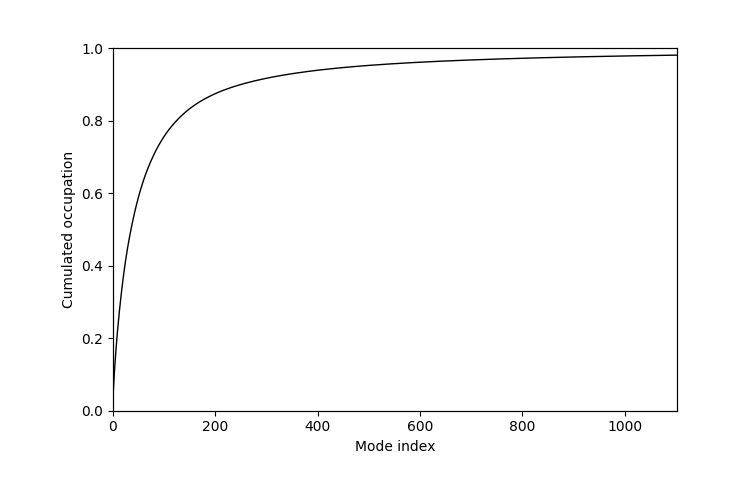
\includegraphics[width=0.4\textwidth]{Figures/vx_cumulated.png}
\end{figure}

\begin{figure}\label{spectral_density}%file plot_spectral_density.py
\caption{Top: Spectral density (intensity) distribution at the source plane. Bottom: Intensity of the first coherent mode at the source plane.}
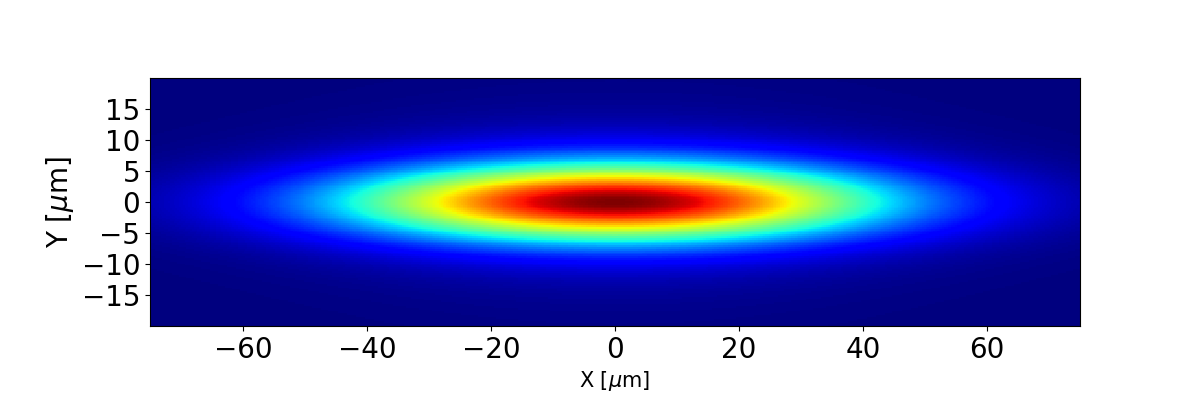
\includegraphics[width=0.45\textwidth]{Figures/spectral_density_upto1099.png}
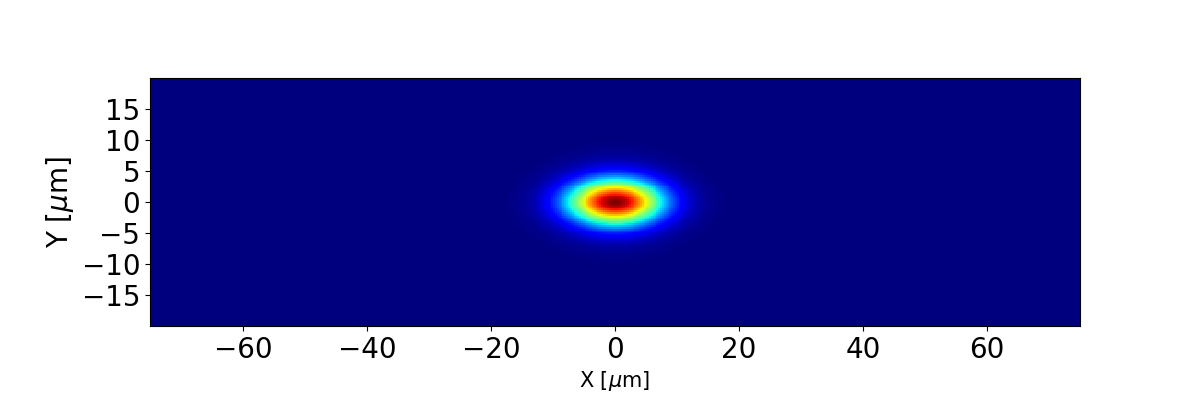
\includegraphics[width=0.45\textwidth]{Figures/spectral_density_upto0.png}
\end{figure}

We then fix a point ``A'' and compute the phase of the CSD up to a given mode $N$. 

\begin{equation}\label{phase_of_W}
\Phi_A(x_1,y_1;z=0,\omega)=\arg[W(x_1,y_1,x_A,y_A;z,\omega)]=\arg[
\sum_{m=0}^{N-1} \lambda_m(\omega)
\phi_m^*(x_1,y_1,\omega)
\phi_m(x_A,y_A, \omega)]
\end{equation}

By selecting different points (A,B,C) and calculating the phase up to a given mode index we observe how vortices appear. They are manifested as points where three colors merge. 



\begin{figure}
A~~~~~~~~~~~~~~~~~~~~~~~~~~~~B~~~~~~~~~~~~~~~~~~~~~~~~~~~~C\\
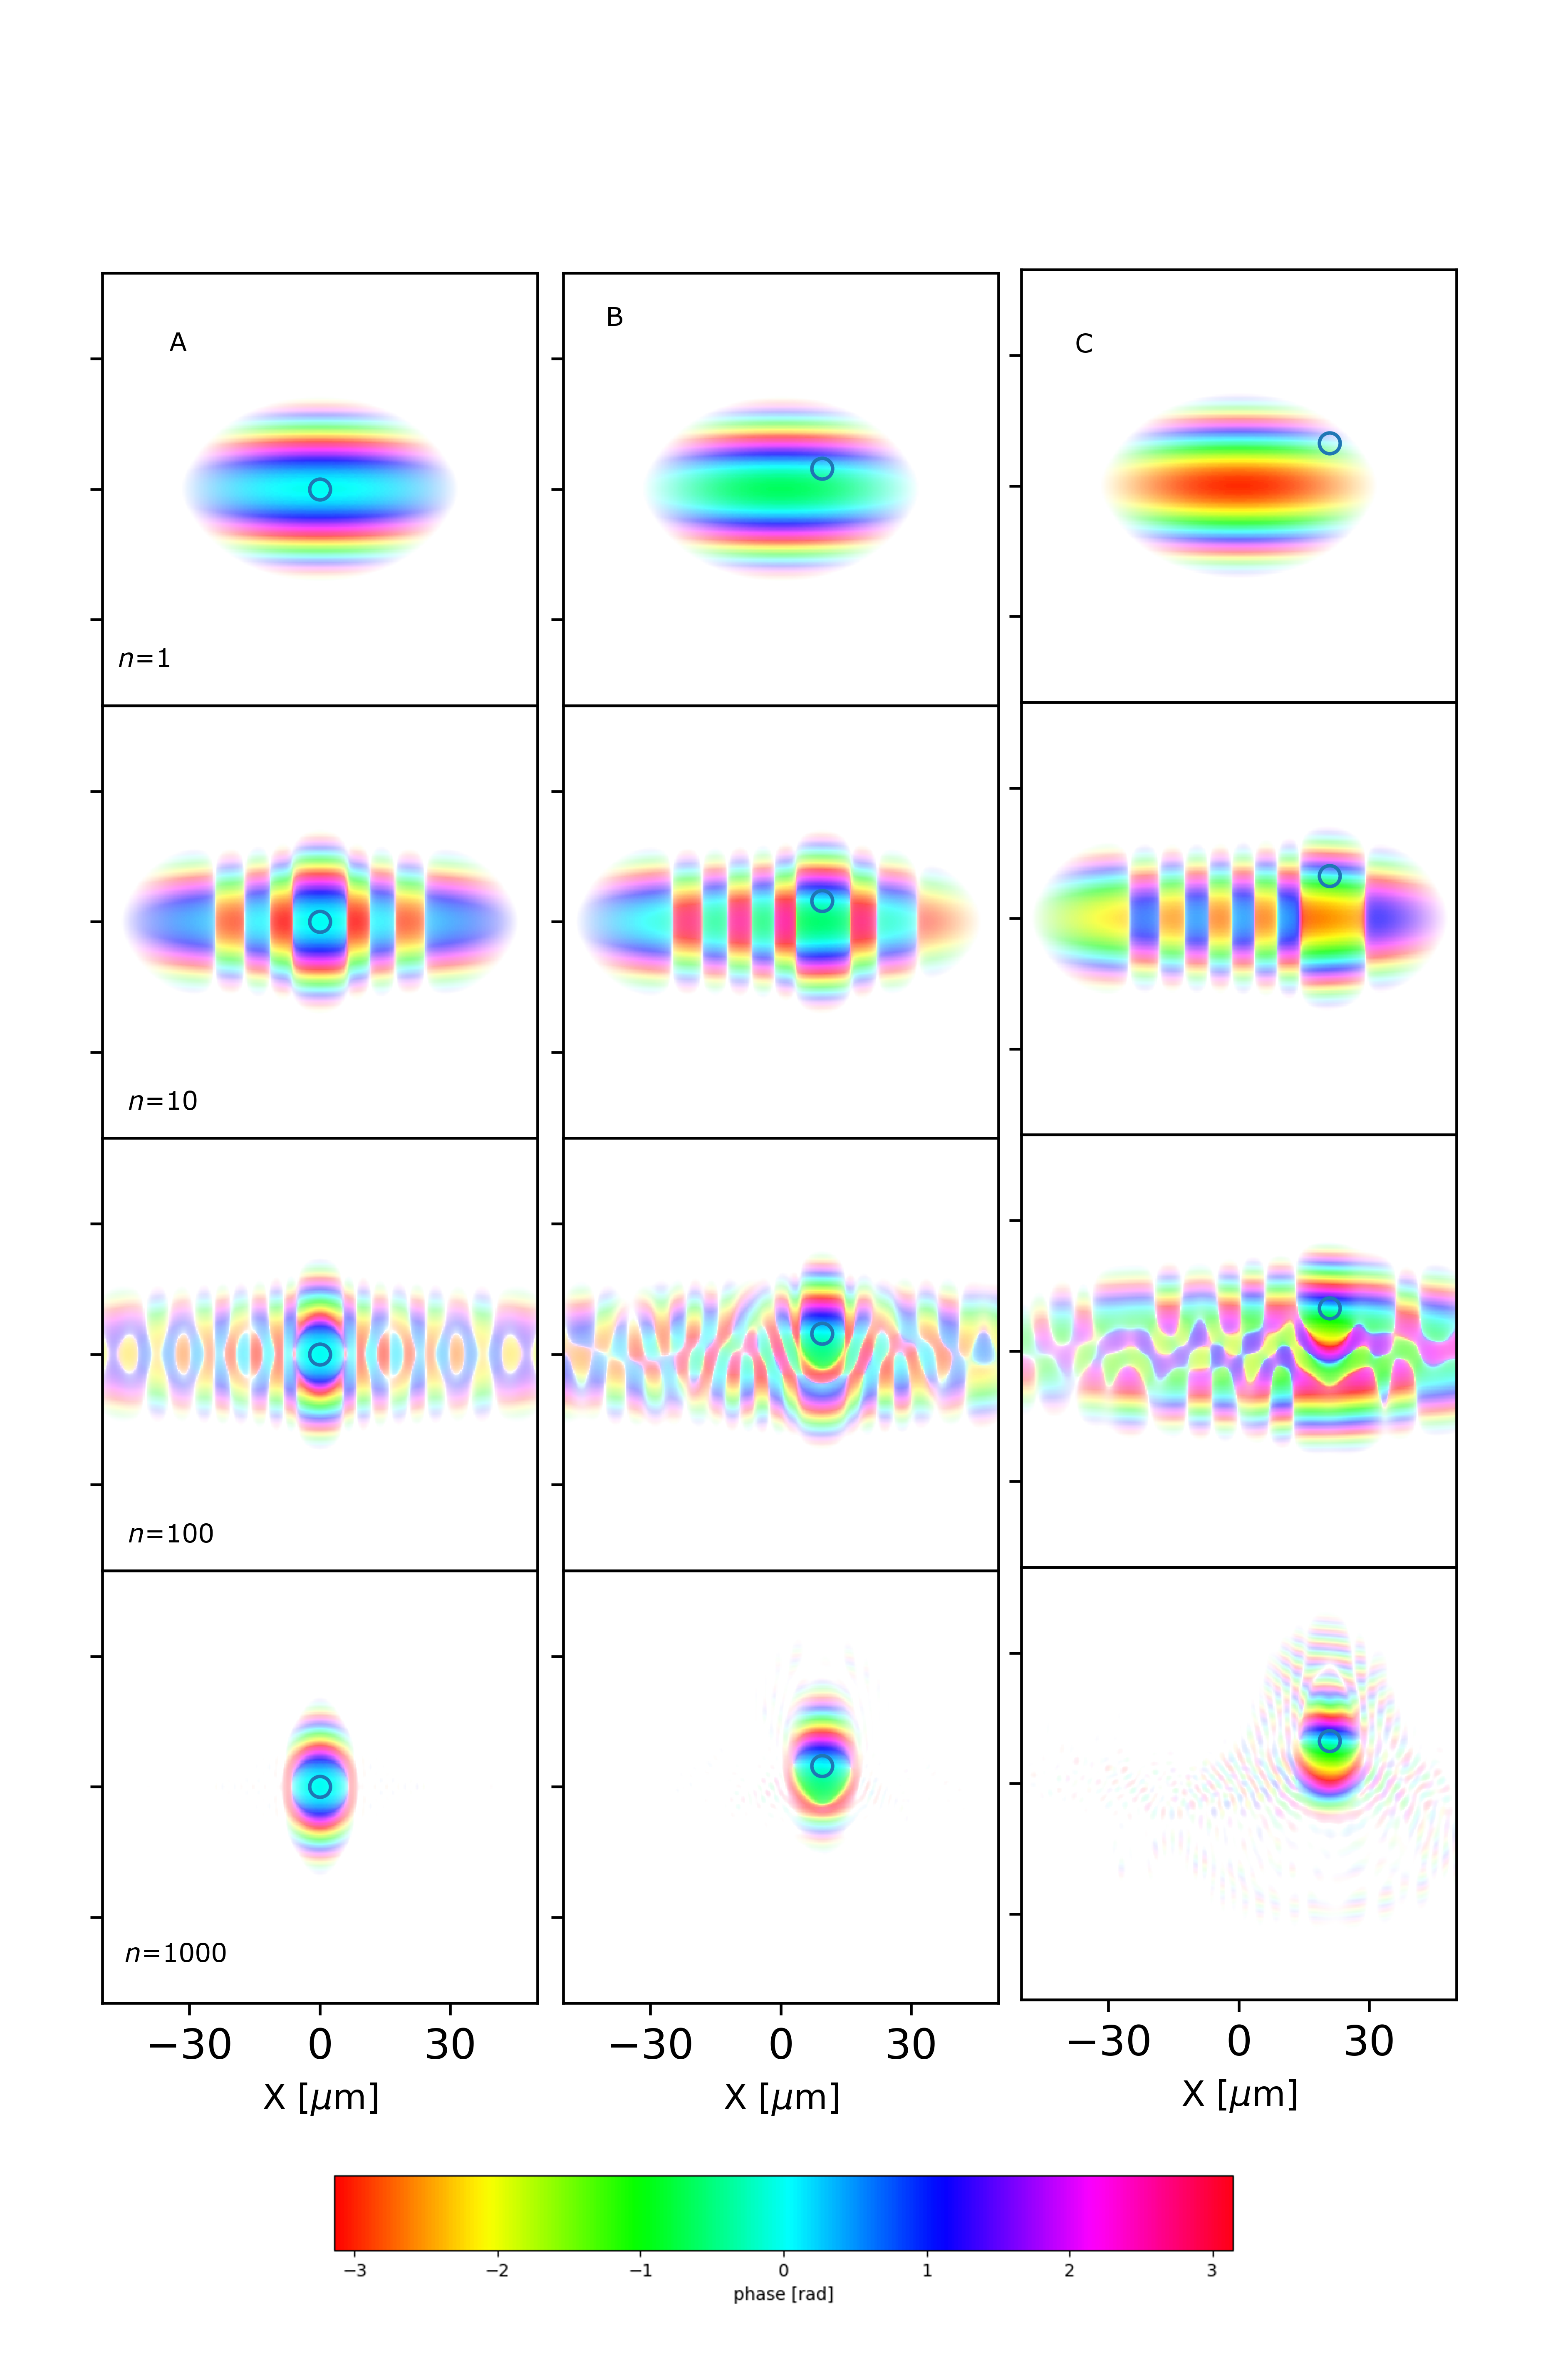
\includegraphics[width=0.95\textwidth]{Figures/vx_id16a_ABC.png}
%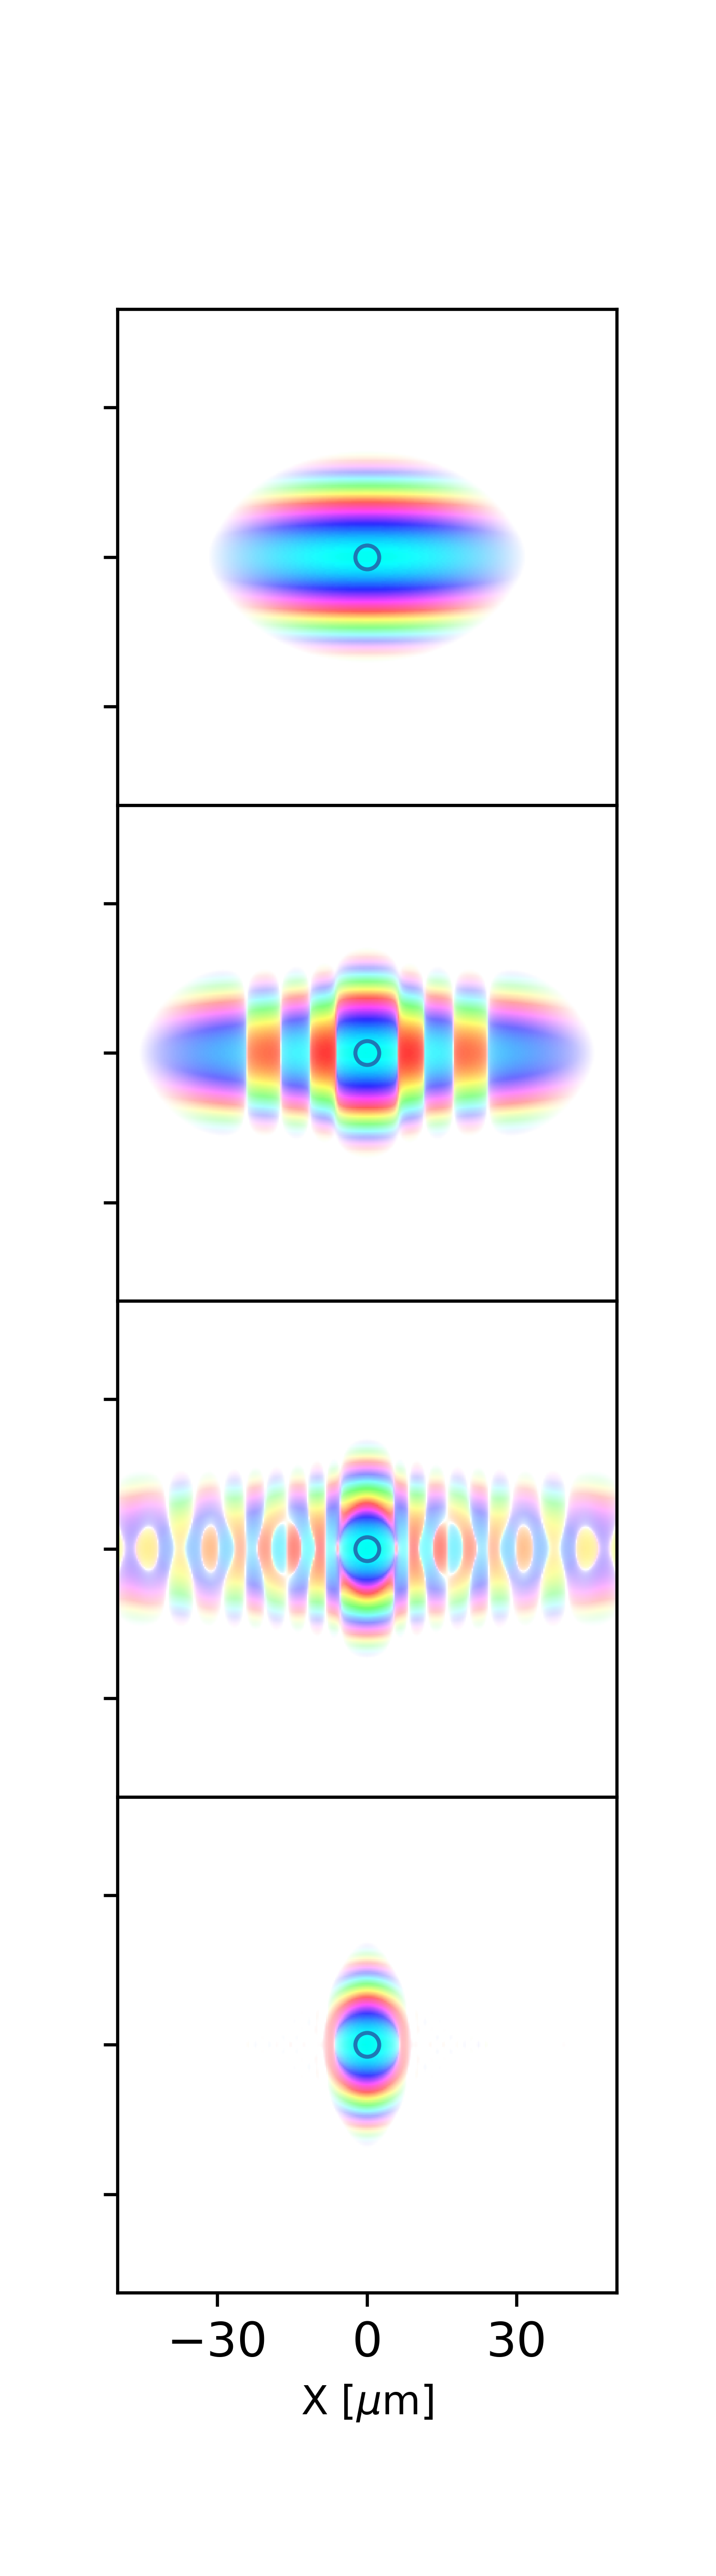
\includegraphics[width=0.32\textwidth]{Figures/vx_id16a_A.png}
%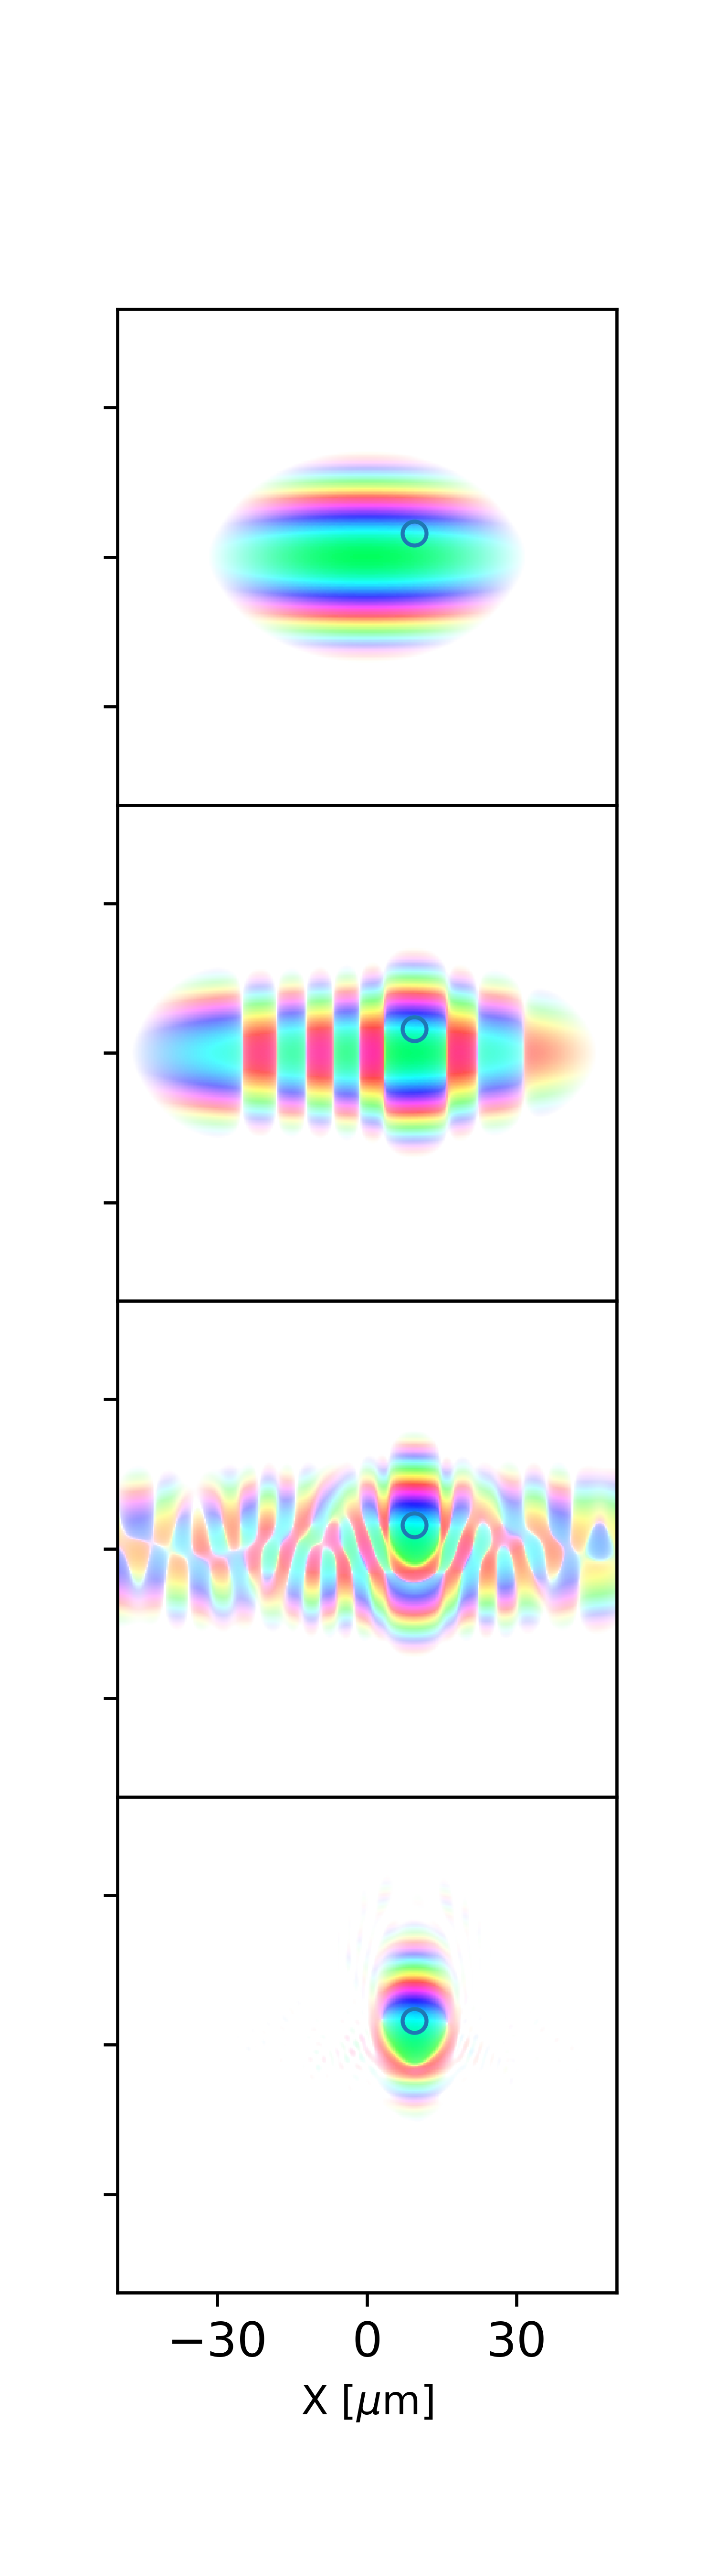
\includegraphics[width=0.32\textwidth]{Figures/vx_id16a_B.png}
%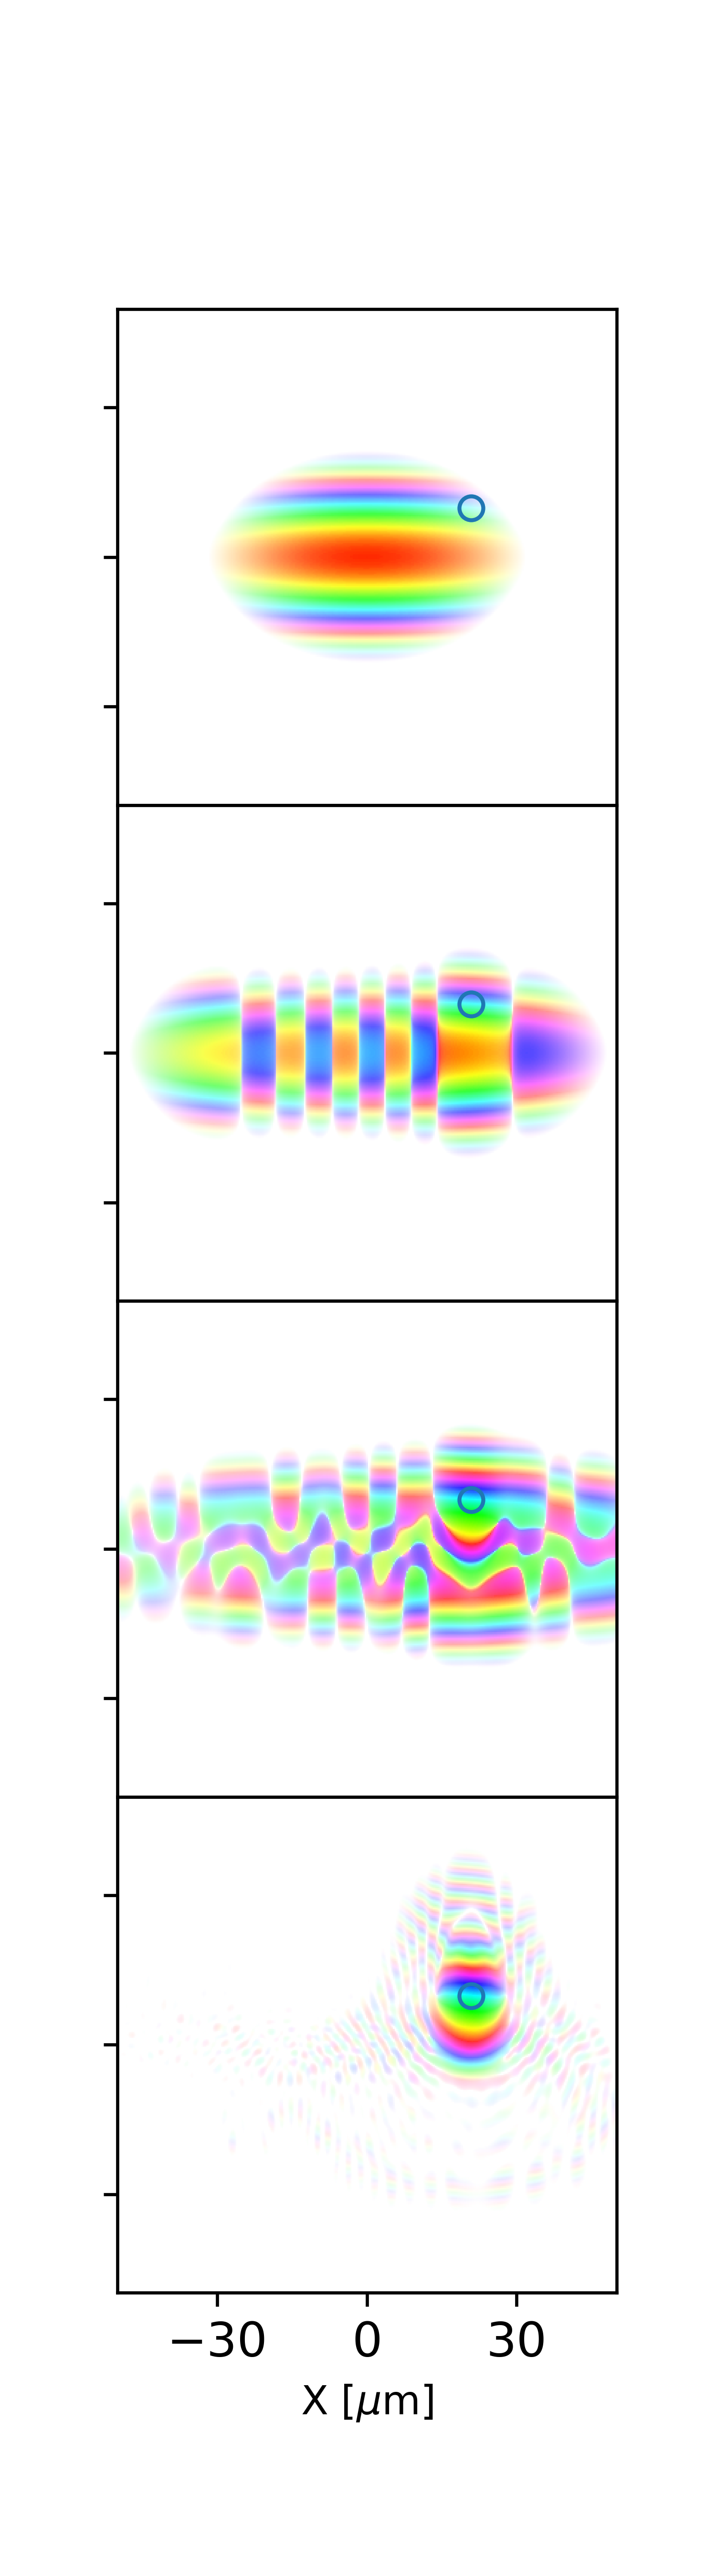
\includegraphics[width=0.32\textwidth]{Figures/vx_id16a_C.png}
%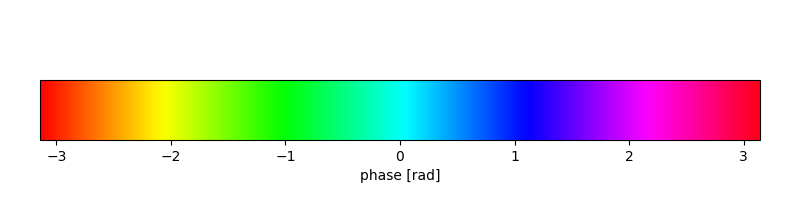
\includegraphics[width=0.95\textwidth]{Figures/color_bar.png}
\end{figure}
 
 
 
 
 
 
 
 \section{Propagated vortices and their effect of reduction of visibility in a Young-like experiment}
 
 
 
 
 
 
 
 
 
 
 
 
 
 
 
 
 
 
 
 
\bibliographystyle{plain}
\bibliography{iucr}

\end{document}
